\documentclass[twocolumn,amsmath,longbibliography,amssymb,superscriptaddress]{revtex4-1}
\usepackage[pdftex]{graphics}
\usepackage{graphicx}
\graphicspath{{figures/}}
\usepackage{hyperref}
\usepackage{xcolor}
\usepackage{physics}
\usepackage{subfig}
\usepackage{bm}
\usepackage{caption}

\newcommand{\carlos}[1]{{\color{red} #1}}
\newcommand{\maria}[1]{{\color{blue} #1}}
\newcommand{\mariac}[1]{{\it\color{cyan}#1}}

	
\begin{document}
		
\title{Something fancy...}
\author{Carlos Ortega Taberner}
\affiliation{Department of Physics, Stockholm University, AlbaNova University Center, SE-106 91 Stockholm, Sweden}
\affiliation{Nordita, KTH Royal Institute of Technology and Stockholm University, SE-106 91 Stockholm, Sweden}

\author{Maria Hermanns}
\affiliation{Department of Physics, Stockholm University, AlbaNova University Center, SE-106 91 Stockholm, Sweden}
\affiliation{Nordita, KTH Royal Institute of Technology and Stockholm University, SE-106 91 Stockholm, Sweden}
\date{\today}
		
\maketitle
	


\section{Introduction}
Topological phases of matter have attracted more and more attention during the last decades, not the least because many more relevant systems have been realized experimentally. 
The early focus was mainly on \emph{topologically ordered} systems \cite{wenbook}, where interaction effects are crucial for stabilizing the phase. 
The most notable examples are the fractional quantum Hall effect~\cite{Tsui1982} and quantum spin liquids~\cite{Balents2010spin}. 
However, since 2005~\cite{kane2005quantum,roy2009topological} the focus has shifted to non-interacting topological phases, which can be characterized in terms of topological invariants~\cite{ryu2010topological}. 
Symmetries are often necessary to protect these topological phases, and determine which distinct topological phases can be realized for a given dimensionality. 

There are a few tools to identify topological phases. 
A very efficient one is the entanglement entropy~\cite{}, which allows one to identify the total quantum dimension of the underlying topological field theory. 
As such, the entanglement entropy can only be used for interacting systems. 
Its main drawback is the fact that it can only provide one of the quantum numbers, and is not able to uniquely determine the topologically ordered phase at hand. 
In addition, it requires a scaling analysis, which can be challenging for strongly correlated systems. 
Another, closely related tool, is the entanglement spectrum (ES), originally introduced for fractional quantum Hall systems~\cite{Li2008entanglement}. 
It was conjectured to provide information about the edge spectrum, which was later shown to be a general feature of ground states with an effective topological field theory description~\cite{Qi2012general}. 
It also proved to be an effective tool for fractional Chern insulators~\cite{Regnault2011fractional} and certain quantum spin liquids~\cite{yao2010entanglement}. \mariac{Others?}

Generically, any of the proposed tools provides some information about the phase naturally, while others seem inaccessible. 
It is not known, whether there exists a method to obtain the full topological data from the ground state. 
For the simplest quantum Hall states, the Laughlin states,  it was shown that the ES does, in fact, contain the full information about the topological phase~\cite{hermanns2011haldane}.
However, it is far from clear if this holds for more complicated/nonabelian states as well.  

Here, we address a much simpler question: what information can be extracted from the ES of \emph{non-interacting} systems?
The latter can be computed very efficiently, using methods developed by Peschel and others~\cite{Peschel2003}. 
It was subsequently shown for topological insulators/superconductors that the ES for (gapped) periodic systems is equivalent to the flat-band energy spectrum of the corresponding system with open boundaries~\cite{Fidkowski2010entanglement}. 
The same correspondence was also found for closely related gapless systems~\cite{matern2018entanglement}
However, even for non-interacting systems, it is unclear which information (beyond the  `edge' spectrum) is encoded in the spectrum. 

In this manuscript, we show that the information about the Berry phase can be completely recovered from the entanglement spectrum and provide a simple formula to do so. 
We relate our results to earlier ones XXX

\emph{Outline of the paper}
\section{Model.}

As a starting point we consider the model in the BDI class used in reference \cite{Song2014} because it is a very simple model which supports topological phases with winding numbers up to $\nu =2$. Additionaly, we include two symmetry breaking terms, $\kappa$ and $\kappa'$, to obtain an even richer phase diagram and show that our results are not limited to any topological class. The Hamiltonian is then given by
\begin{align}
H =& \sum_{i\alpha,j\beta} c_{i\alpha}^\dagger H_{ij,\alpha \beta} c_{j\beta} \\
H_{ij} =& (m \sigma_x + \kappa \sigma_z)\delta_{ij}  + \frac{1}{2i}\kappa'\sigma_z (\delta_{i-j,1}-\delta_{i-j,-1})\\
&+ \frac{1}{2} t \left[(\sigma_x + i \sigma_y)\delta_{i,j+1} + (\sigma_x - i \sigma_y) \delta_{i,j-1} \right] \\
&+  \frac{1}{2} t' \left[(\sigma_x + i \sigma_y)\delta_{i,j+2} + (\sigma_x - i \sigma_y) \delta_{i,j-2} \right],
\label{bdi_model}
\end{align}
with the corresponding Bloch Hamiltonian being
\begin{align*}
H(k)=&\mqty( \kappa + \kappa' \sin(k) & t' e^{i2k} + t e^{ik}+m \\t' e^{-i2k} + t e^{-ik}+m & -\kappa-\kappa' \sin(k)  ) \\
=& (t' \cos(2k)+t\cos(k)+m)\sigma_x \\
&+ (-t' \sin(2k)-t\sin(k))\sigma_y + (\kappa+\kappa'\sin(k)) \sigma_z.
\end{align*}
For $\kappa = \kappa' = 0$ this Hamiltonian has the following symmetries
\begin{alignat*}{2}
&T = \mathcal{K} ; \quad &&T H(-k) T^{-1} = H(k) \\
&C = \sigma_z\mathcal{K} ; \quad &&C H(-k) C^{-1} = -H(k) \\
&S = \sigma_z ; \quad &&S H(k)S^{-1} = -H(k) 
\end{alignat*}
and therefore it is in the BDI class, where the system has the phase diagram shown in Fig.\ref{bdi_phase_diagram} for $t=1$. We also show cuts with the transitions $\nu = 2 \rightarrow 0$ and $\nu = 1 \rightarrow 2$ for different values of $\kappa,\kappa'$.  For $\kappa' \neq 0$ only $C$ is preserved and the system belongs to the $D$ class. The $Z$ invariant transforms into a $Z_2$ invariant and the original $\nu = 2,0$ phases become equivalent. For $\kappa \neq 0$ only $T$ is preserved and the system is in the trivial AI class, where all zero-energy modes split.
\begin{figure}[h!]
\centering
\makebox[0pt]{
\subfloat[$t = 1,\kappa =\kappa'=0$]{
  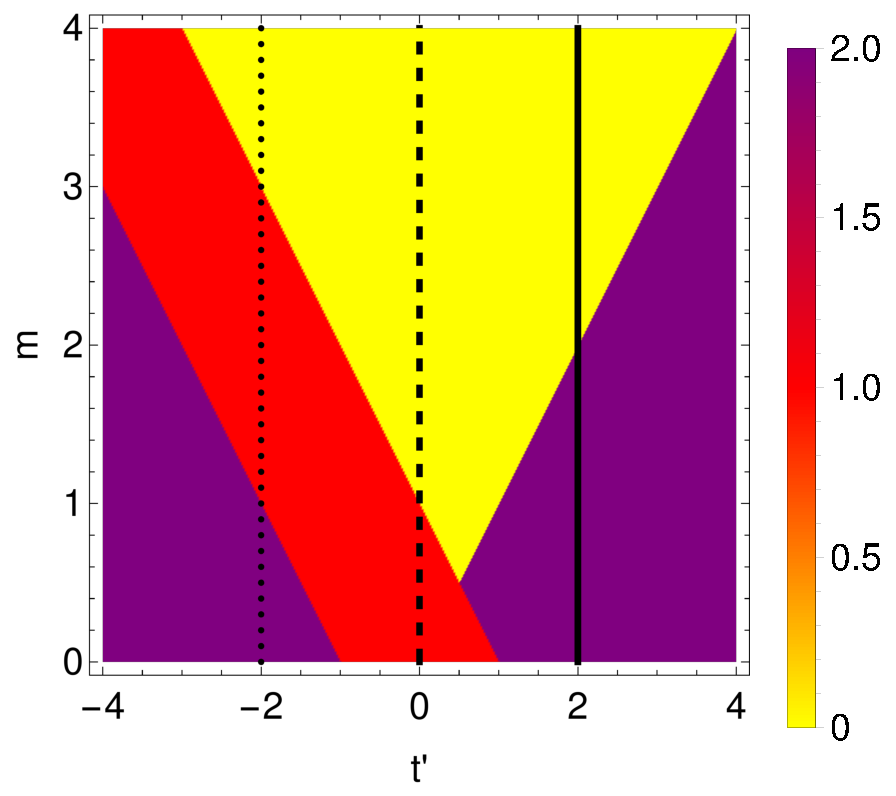
\includegraphics[width=45mm]{phase_diagram2.pdf}
}}\hspace{0mm}

\makebox[0pt]{
\subfloat[$t = 1,t'=1$, \, $\kappa =\kappa'=0$]{
  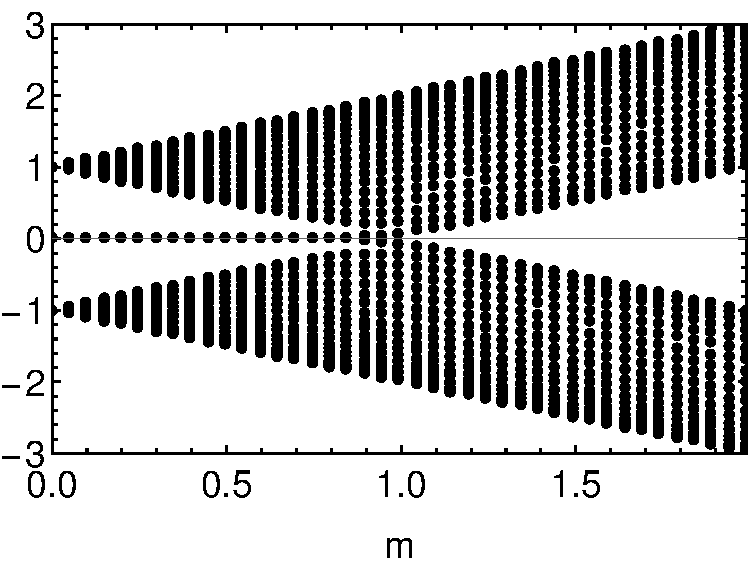
\includegraphics[width=35mm]{1_a.pdf}
}
\subfloat[$t=1,t'=1$, $\kappa = 0.3, \kappa'=0$]{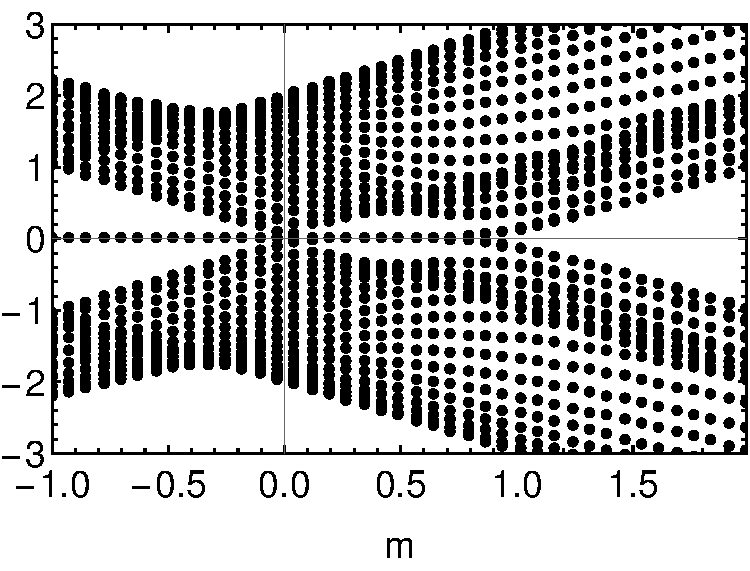
\includegraphics[width=35mm]{1_b.pdf}
}
}\hspace{0mm}

\makebox[0pt]{
\subfloat[$t = 1,t'=1$, $\kappa = 0,\kappa'=0.3$]{
  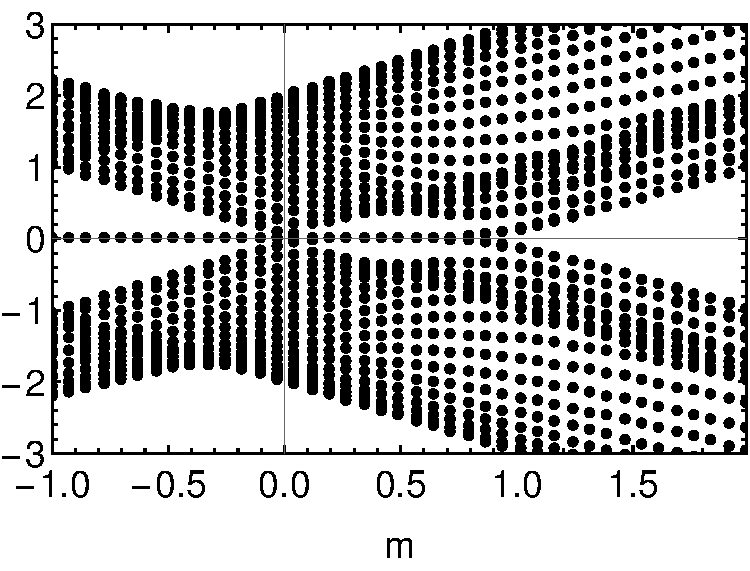
\includegraphics[width=35mm]{1_b.pdf}
}
\subfloat[$t=1,t'=1$, $\kappa = 0.3,\kappa'=0.3$]{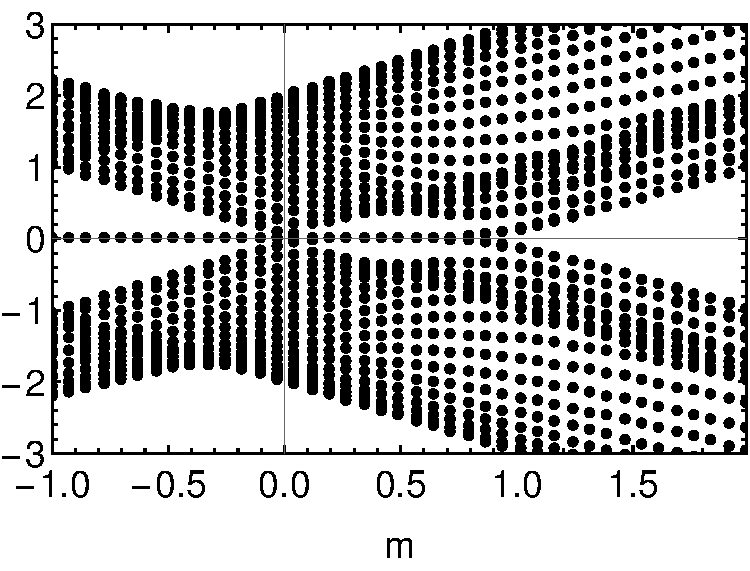
\includegraphics[width=35mm]{1_b.pdf}
}
}
\caption{Phase diagram for the system in the $BDI$ class showing the winding number of each region and surface energy spectrum for two different cuts in the phase diagram for different values of $\kappa,\kappa'$. \carlos{I'm not sure what to include here.}}
\label{bdi_phase_diagram}
\end{figure}

\section{Zak phase and Entanglement spectrum}
Consider a quadratic Hamiltonian in one dimension
\begin{equation}
\mathcal{H} = \sum_{ij,\alpha\beta} c_{i\alpha}^\dagger H_{ij,\alpha \beta}c_{j\beta}.
\end{equation}
We can obtain the single-particle eigenstates as
\begin{align*}
\sum_{j\beta}H_{ij,\alpha\beta} u^{p\mu}_{j\beta} = E_{p\mu} u_{i\alpha}^{p\mu},
\end{align*}
where $[U]_{j\beta,p\mu} = u^{p\mu}_{j\beta}$ is the unitary matrix that diagonalizes $H$. The polarization can be obtained as the many-body average of position operator, regularized for periodic boudnary conditions \cite{Resta1997}
\begin{align*}
\expval{X} = -\frac{L}{2\pi} \rm{ Im\, Ln }\bra{\Psi_0}e^{-i \frac{2\pi}{L}\hat{X}}\ket{\Psi_0},
\end{align*}
where $\ket{\Psi_0}$ is the many-body ground state and $\hat{X}$ is the sum of all the single-particle position operators.
Using that the ground state is a Slater determinant of the single-particle eigenstates, $\ket{u^{p\mu}}$, it can be rewritten as
\begin{align*}
\expval{\hat{X}} = -\frac{L}{2\pi} \rm{Im \, Ln}\, {\rm det} \, \tilde{S},
\end{align*}
where the matrix $\tilde{S}$ is obtained from another matrix S with elements
\begin{equation}
S_{p\mu,q\nu} = \sum_{j\alpha}u^{p\mu\, \ast}_{j \alpha} e^{-i\frac{2\pi}{L}j}u^{q\nu}_{j \alpha}
\end{equation}
by restricting it to the space of occupied single-particle states. The Zak phase can now be obtained as
\begin{equation}
\gamma = \expval{\hat{X}}\frac{2\pi}{L} + \frac{1}{2}
\end{equation}
\carlos{There is an extra 1/2 factor compared to Kivelson's formula which I don't know where it is coming from.}
The correlation function in position space is given by
\begin{align*}
C_{ij}^{\alpha \beta} = \expval{c_{i\alpha}^\dagger c_{j\beta}}.
\end{align*}
In terms of the fermions that diagonalize the Hamiltonian, 
\begin{align*}
& \gamma_{i\alpha} = \sum_{j\beta}u_{j\beta}^{i\alpha \, \ast} c_{j\beta} \\
& c_{i\alpha} = \sum_{j\beta} u^{j\beta}_{i\alpha} \gamma_{j\beta}
\end{align*}
we have
\begin{align*}
C_{ij}^{\alpha \beta} =& \sum_{pq,\mu\nu} u^{q\nu }_{j\beta} u^{p\mu \, \ast}_{i\alpha} \expval{\gamma^\dagger_{p\mu} \gamma_{q\nu} } \\
=&  \sum_{p\mu} u^{p\mu }_{j\beta} u^{p\mu \, \ast}_{i\alpha} \expval{\gamma^\dagger_{p\mu} \gamma_{p\mu} } \\
=&  \sum_{p\mu} u^{p\mu }_{j\beta} u^{p\mu \, \ast}_{i\alpha} [1-{\rm sign}(E_{p\mu})]/2.
\end{align*}
The first term is simply a kronecker delta between both sets of indeces. The second term can be rewritten as
\begin{align*}
UD(\abs{D})^{-1}U^\dagger =& UD(D^2)^{-1/2}U^\dagger \\
=& U D U^\dagger (U D^2 U^\dagger)^{-1/2} \\
=& H(H^2)^{-1/2},
\end{align*}
where $D$ is the diagonal Hamiltonian, $H=UDU^\dagger$. Finally the correlation function can be obtained in position space as
\begin{align*}
C_{ij}^{\alpha \beta} =& \frac{1}{2}\left[I - H/ (H^2)^{-1/2} \right]_{ij, \alpha \beta}
\end{align*}
The entanglement spectrum (ES) is then obtained as the spectrum of the subsystem correlation function obtained after bisecting the system into two equal parts. 

In the ES we can differentiate between two types of eigenvalues, which we denote by $\xi$. The ones at $\xi_b = 0,1$ correspond to bulk states while for the ones in between, $0<\xi_{l,r}<1$, we find their correspondent eigenstate localized in either the left, $\xi_l$, or right, $\xi_r$, virtual edge \cite{Peschel2008}. 

\section{Homogeneous system}

\subsubsection{One edge mode case}

For symmetry-protected topological systems in one dimension there is a well-known relation between ES and the Zak phase. The Zak phase, which is quantized, is zero whenever there is an even number per edge of eigenvalues at $\xi = 1/2$, and $\pi$ when the number is odd. Beyond symmetry protected systems, there was observed that in the fully dimerized SSH chain, with only a single mode present in the ES, the Zak phase is equal to the midgap eigenvalue \cite{Ryu2006}. For slighly more complex ES it has been shown that the Zak phase follows the midgap eigenvalues qualitatively \cite{Huang2012,Huang2012-2}. It is known \carlos{Cite peschel} that the entanglement energies of 1D chains are equispaced sets of distinct values. The first result we show is that in simple systems like the SSH chain, where there is only one "distinct" mode, one can obtain the Zak phase by ordering the eigenvalues of the ES, $\xi_1 < \xi_2 < ...$, and computing
\begin{equation}
\chi = \frac{1}{2}\left(\sum_j (-1)^j \xi_j+N_A\right) \, {\rm mod} \, 1,
\label{eqplusminus}
\end{equation}
where $N_A$ is the number of electrons in the ground state in region A, which in the thermodynamic limit fulfills
\begin{equation}
\lim_{L \rightarrow \infty} \gamma = \lim_{L \rightarrow \infty} \chi.
\end{equation}
In the case where there is only one finite eigenvalue in  the ES, like in the fully dimerized limit of the SSH chain, we recover the equality between the midgap eigenvalue and the Zak phase. In Fig.\ref{huang} we show the case were it is not fully dimerized. We see in Fig.\ref{huang}.a that even though in the symmetry protected case the ES has finite eigenvalues in the trivial phase these are double-degenerate so that they cancel each other. In the case where we break the symmetry we see that there is one main midgap eigenvalue, so that the Zak phase follows it very closely, but as the midgap eigenvalue approaches the bulk the contribution from the other modes becomes more relevant and the Zak phase, and therefore $\chi$, start to deviate from the midgap eigenvalue.
\begin{figure}[h!]
\centering
\makebox[0pt]{
\subfloat[$t = 1,t'=0$, \, \,$\kappa =\kappa'=0$]{
  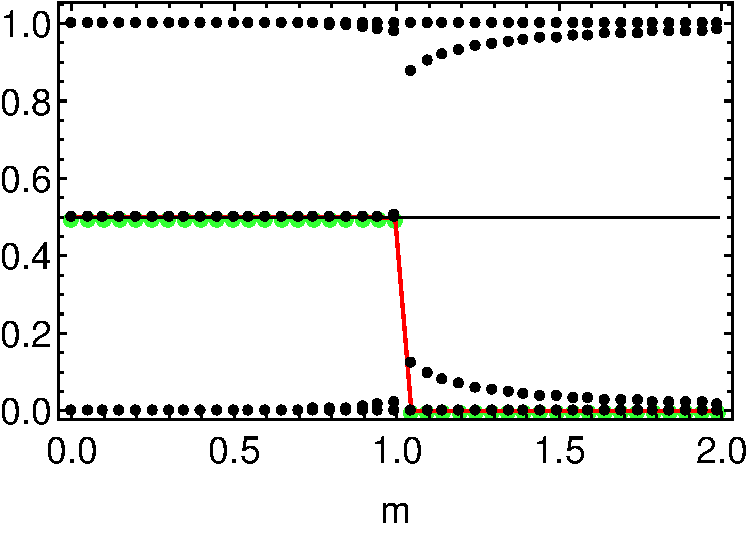
\includegraphics[width=35mm]{2_a.pdf}
}
\subfloat[$t=1,t'=0$, $\kappa = 0.3, \kappa'=0$]{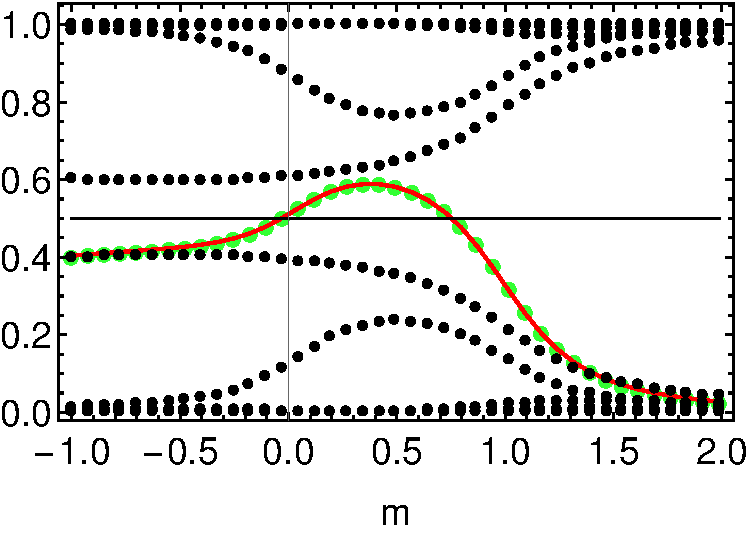
\includegraphics[width=35mm]{2_b.pdf}
}
}
\caption{Phase diagram for the system in the $BDI$ class showing the winding number of each region and surface energy spectrum for two different cuts in the phase diagram for different values of $\kappa,\kappa'$.}
\label{huang}
\end{figure}

\subsubsection{Localization dependent charges}

In order to generalize this to more complex systems one needs to know how to properly assign this $\pm 1/2$ charge to each entanglement mode. This is done according to their localization classification, so we have
\begin{equation}
\chi = \frac{1}{2} \left( \sum_{i\in r}\xi_i-\sum_{i\in l}\xi_i \pm \sum_{i\in b}\xi_i  + N_A \right) \quad {\rm mod} \quad 1,
\label{loceq}
\end{equation}
the charge of the bulk modes so far is irrelevant since their eigenvalue is 1 in the thermodynamic limit, but in the next section we will have to take a closer look at it.  In the case the spectrum is double degenerate the left and right edge states might mix but one will always classify oneof the pair as left and the other one as right states, which is why the expression Eq.~\eqref{eqplusminus} simplifies so much. Even in the case where the degeneracies are broken the pairs of entanglement modes split in the same way (all left modes go up, right ones go down, or the other way around) so that the formula still applies as long as there are no crossings. This is however not the case when the degeneracies are higher than two-fold, or when we have more modes present that can cross. In order to always obtain localized modes we diagonalize instead $C_A + \lambda C_A\hat{X}C_A$, where $\hat{X}$ is the position operator and $\lambda$ is a small parameter that vanishes in the thermodynamic limit. This relation between the Zak phase and the entanglement spectrum is a consequence of an identity between the Zak phase and the many-body entanglement spectrum previously found for infinite chains \cite{Zaletel2014}. In Appendix A (\carlos{I have to take a look at it again}) we modified this derivation to account for the periodic boundary conditions we use and show how their result reduces to Eq.~\eqref{loceq} when expressing it in terms of the ES.

In Fig.\ref{2},a,b. we show an example that highlights the importance of the localization structure of the ES. Two ES that seem at first very similar result in very different Zak phases. This happens because of how the two symmetry breaking terms split the four-fold degenerate midgap states. While $\kappa'$ splits them into two two-fold degenerate pairs whose contribution cancels, $\kappa$ split thems into two $left-left$ and $right-right$ pairs, with a finite contribution to the Zak phase. In Fig.\ref{2},c,d. we also show the $\nu = 2 \rightarrow 1$ cut in the phase-diagram, to illustrate a more complex ES. 

One drastic example of this can be seen in figure \ref{old} , where two ES that look almost identical result in a very different Zak phase. \carlos{This was an old plot I don't know if we want to keep or not}

\begin{figure}[h!]
\centering
\makebox[0pt]{
\subfloat[$t = 1, t' = 2,$   $\kappa =0.3, \kappa' = 0$]{
  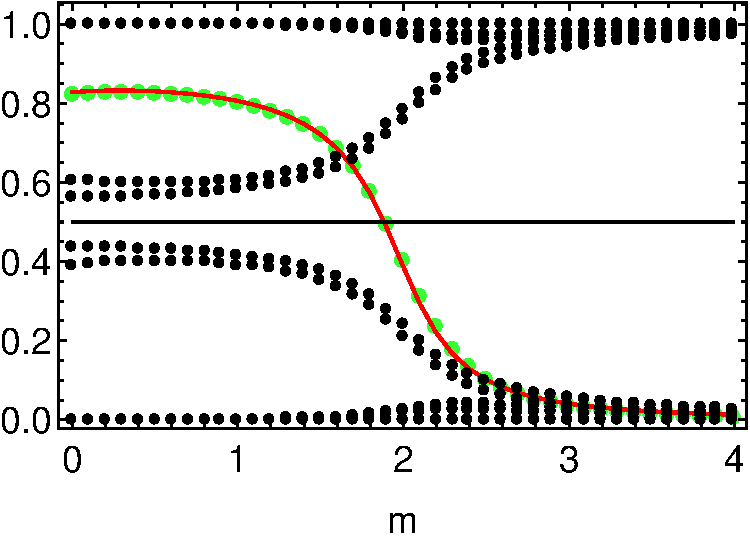
\includegraphics[width=35mm]{3_a.pdf}
}
\subfloat[$t = 1, t' = 2,$ $\kappa = 0, \kappa' = 0.3$]{
  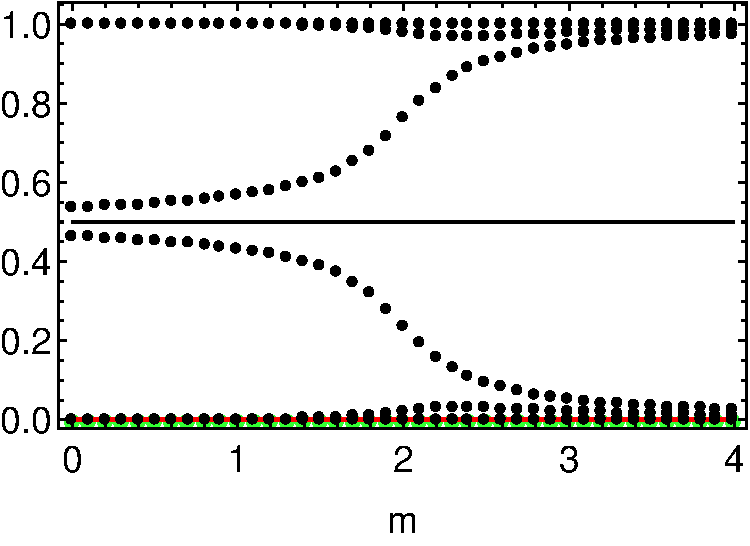
\includegraphics[width=35mm]{3_b.pdf}
}
}\hspace{0mm}

\makebox[0pt]{
\subfloat[$t = 1, t' = -2,$ $\kappa = 0.3, \kappa' = 0$]{
  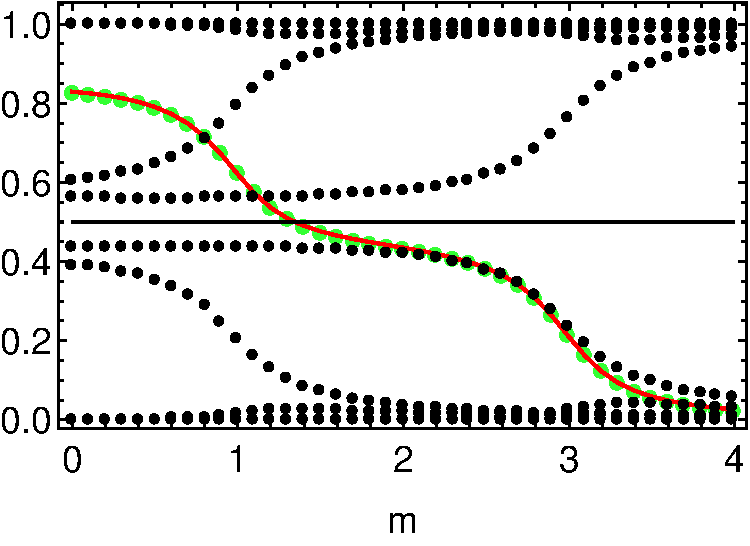
\includegraphics[width=35mm]{3_c.pdf}
}
\subfloat[$t = 1, t' = -2,$ $\kappa = 0, \kappa' = 0.3$]{
  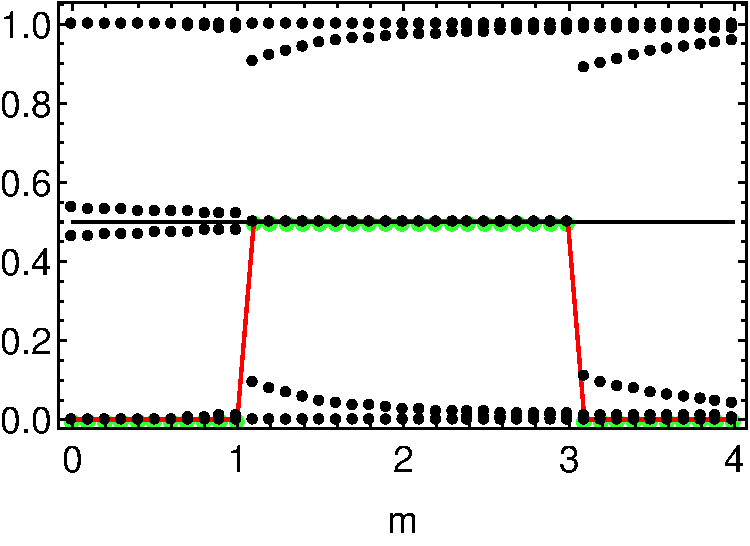
\includegraphics[width=35mm]{3_d.pdf}
}
}
\caption{Entanglement spectrum (black), $\chi$ (green) and $\gamma$ (red)  }
\label{2}
\end{figure}




\section{Inhomogeneous systems}

\subsubsection{Simple case, continuous ES.}

In reference \cite{Zaletel2014} translational invariance was used to derive Eq. \ref{zaletel} in Appendix A. Say we break translational invariance by adding weak disorder to the system. This will modify slightly the entanglement spectrum but not the charge assignment. Without translational invariance the entanglement spectrum will depend on where is the cut placed on the ring, even though the ground state, and therefore the Zak phase, will not. The first quantity one can construct that is cut-independent is the cut-average of $\chi$. Naively one would define
\begin{equation}
\bar{\chi} = \frac{1}{L}\sum_{s=1}^L \chi_s
\label{batcutavg}
\end{equation}
where
\begin{equation}
\chi_s = \frac{1}{2} \left( \sum_{i\in r}\xi^s_i-\sum_{i\in l}\xi^s_i \pm \sum_{i\in b}\xi^s_i  + N_A \right) \quad {\rm mod} \quad 1,
\end{equation}
is defined for cuts at $s$ and $s+L/2$. However the average of a circular quantity is not well defined. The reason we took the modulo 1 was to get rid of the bulk contribution, which should vanish in the end result anyway. If we take the modulo 1 after averaging we still might have an issue due to the bulk classification being inconsistent. A bulk mode near the center of A, at $L/4$, might cross $L/4$ at different cuts, changing its assigned charge. The bulk contribution will not be constant across cuts and that will lead to errors when averaging. 

One can get away with expression Eq.~\eqref{batcutavg} in a few cases. For a system with a continuous position-dependent Hamiltonian in a trivial phase, $\chi_s$ should also be continuous. This tell us how we have to perform the cut-average. Even when discontinuities are present as long they are weak enough so that we still can tell when $\chi_s$ crosses $0,1$, we can use this information to perform the cut average. In the case that the width of $\chi_s$ is lower than 1 one can select the range of values so that $\chi_s$ does not cross the "$0,1$" line and then average. We show this in Fig.\ref{inh}.a for a system with disorder on $\kappa_s$. Note that even though we have random disorder the ES, and therefore $\chi_s$ shows some sign of continuity so that the cut-averaged can be performed this way even for relatively strong disorder.



\begin{figure}[h!]
\centering
\makebox[0pt]{
\subfloat[$\kappa_s$]{
  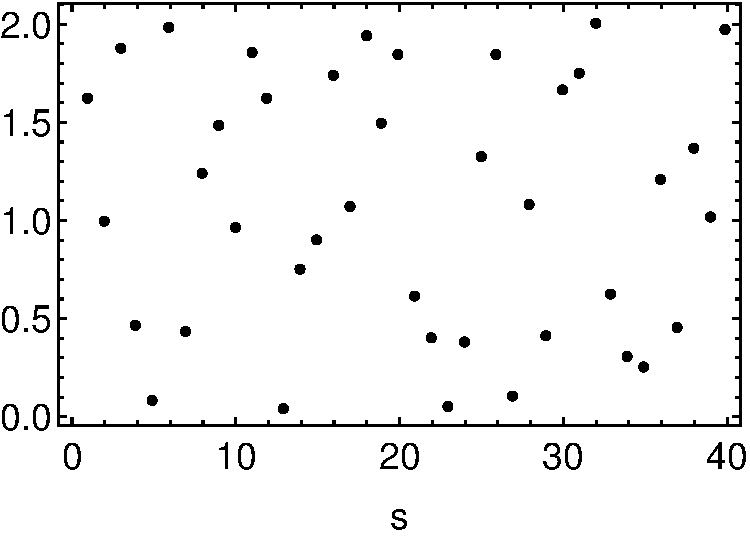
\includegraphics[width=40mm]{4_c.pdf}
}
\subfloat[$t=1,t'=2,m =1$ ]{
  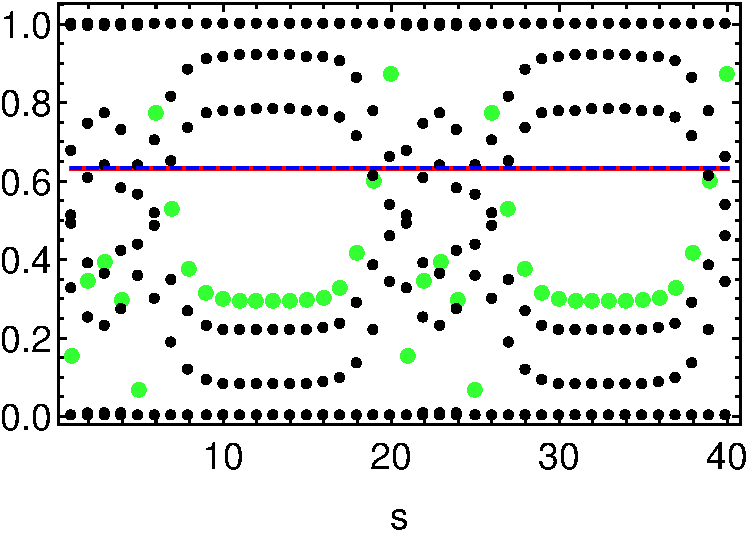
\includegraphics[width=40mm]{4_d.pdf}
}
}\hspace{0mm}

\makebox[0pt]{
\subfloat[$\kappa_s$]{
  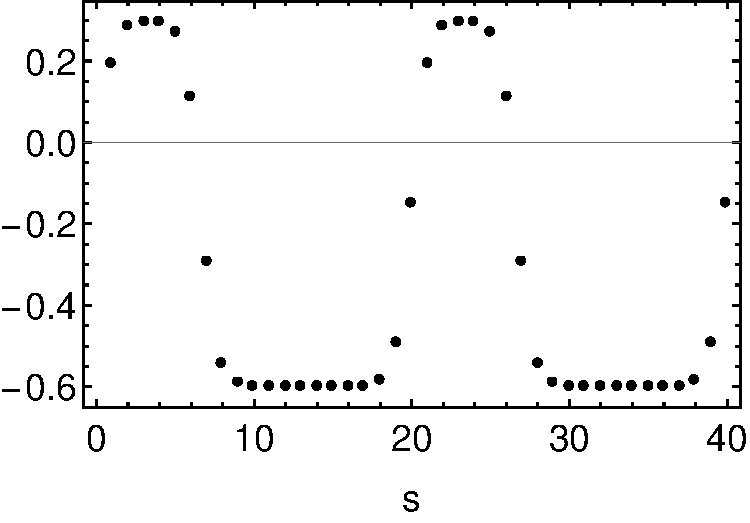
\includegraphics[width=40mm]{4_a.pdf}
}
\subfloat[$t=1,t'=2,m =1$]{
  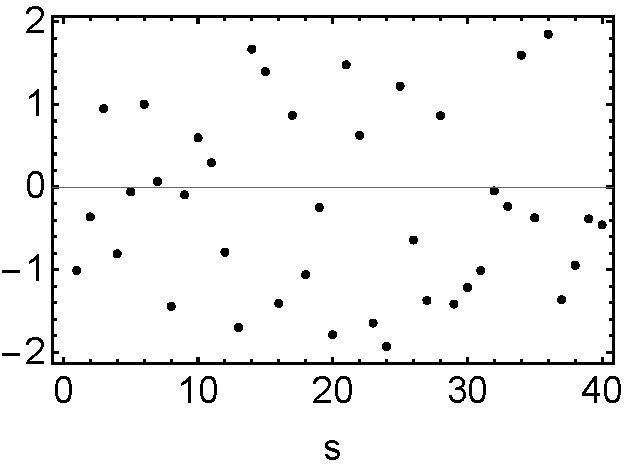
\includegraphics[width=40mm]{4_b.pdf}
}
}
\label{inh}
\end{figure}

In the case where $\chi_s$ is continuous but the width is larger than 1 can construct a new quantity $\chi_s'$ that is not defined modulo 1, by extending the range of $\chi_s \, {\rm mod} \, 1$ every time it crosses $0$ or $1$, such that
\begin{equation}
\chi_{s+1}' = {\rm Min}\{\chi'_{s+1}-\chi'_s,\chi'_{s+1}-\chi'_s+1,\chi'_{s+1}-\chi'_s-1\}
\end{equation}
where at each step $\chi_{s+1}'$ is chosen by minimizing the absolute value of the difference. In Fig.\ref{inh}.b we show an example of this. In Fig.\ref{disorder} we show $1-\expval{\chi_s}_{\rm cuts}/\gamma$ for different system lengths for system with weak disorder, as well as the disorder average of $1-\chi_0/\gamma$. We observe that both averages lead to the same difference, which scales as $O(L^{-2})$ (\carlos{I have to redo de plot, maybe scaling is different}), vanishing in the thermodynamic limit. The fact that both methods lead to the same error suggests that it comes strictly from a systematic finite size error in the computation of either the Zak phase or the ES which is system-independent. 

\begin{figure}[h]
\centering
\makebox[0pt]{
\subfloat[$t = 0, t' = 2, \kappa = 0.3$]{
  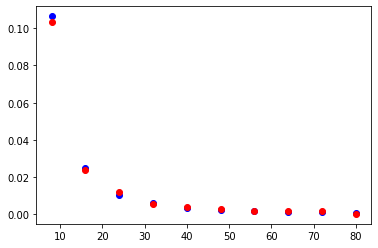
\includegraphics[width=65mm]{scaling_cut_disavg.png}
}
}
\caption{\carlos{Redo}}
\label{disorder}
\end{figure}

\subsubsection{Wannier states, L/4 crossing fix}

In a general case where the discontinuities are too strong and the discussed above does not apply one has to take a closer look into the bulk states to ensure a consistent classification. As we mentioned above the bulk states farthest away from the edges are the problematic ones. They are also the ones best approximated by the Wannier states obtained from the chain with periodic boundary conditions as the eigenstates of 
\begin{equation}
C\hat{X}_{\rm PBC}C
\end{equation}
where $\hat{X}_{\rm PBC} = \exp\{i 2\pi \hat{X}/L\}$. Similar to when we go through different cuts labeled by $s$, we now consider the Wannier states dependent on where we define our lattice site 1, shifted by $s$. The obtained Wannier states for $s$ and $s+1$ will be therefore exctly the same, but shifted one lattice site. By considering their average position $\expval{\hat{X}_{PBC}}_{i,s}$ we can define a set of $2L$ Wannier states that depend continuously on $s$ (provided that the Hamiltonian is continuous). These Wannier states are then a good approximation for the Bulk states of $C_A$ we find for the different cuts. Consider now the quantity $\sum_i\expval{\hat{X}}_{i,s}$. So far everything was $s$ independent as our system was periodic, but by considering the operator $\hat{X}$ we introduce an unphysical boundary so that it will depend on where we put the first and last sites. If the states do not cross this unphysical boundary then $\sum_i\expval{\hat{X}}_{i,s} = \sum_i\expval{\hat{X}_{\rm PBC}}_{i,s} $ and it will be a constant. However, when a Wannier state crosses the boundary we obtain the same constant plus $L$. If we put this boundary at $L/4$ the object 
\begin{equation}
\frac{1}{L}\left(\sum_i\expval{\hat{X}}_{i,s}-\sum_i\expval{\hat{X}}_{i,0}\right)
\end{equation}
will be 1 (0) when a states has crossed the boundary or 0 (-1) when it has not, depending on the number of states in A at $s=0$, which we take as reference. Depending which state we take as reference will introduce a global integer shift for all cuts, so it is not relevant as it will go away after we average and take the modulo 1. By adding this term to our cut-average we will compensate for when our bulk state in the middle of A crosses $L/4$ and its charge changes. Leading to a continuous $\chi_s$ which can be averaged. In Fig.\ref{wan} we show how this works for one case. In Fig.\ref{wan}.a we show the expectation value of the position operator for both the entanglement eigenstates (in black) and the Wannier states (in red) for different cuts. In Fig.\ref{wan}.b and c we show $\chi_s$, which displays jumps due to a bulk state crossing $L/4$, and 
\begin{equation}
\chi_s' = \chi_s + \frac{1}{L}\left(\sum_i\expval{\hat{X}}_{i,s}-\sum_i\expval{\hat{X}}_{i,0}\right),
\end{equation}
where the position is defined in $[-3L/4,L/4]$ to correctly compensate for these jumps. This method conceptually works perfectly whenever the bulk states of the ES match the Wannier states, i.e. in the thermodynamic limit, but it is not clear what the small parameter is. It depends on the $\lambda$ used (it should be small enough to not affect ES but large enough to localize the ES eigenstates) but also on the model. Models with longe-range hopping, for example, lead to a higher number of edge modes in the ES which makes the effect of the edge go deeper into the bulk. 
\carlos{We should think again if there is a better method to get this}

\begin{figure}[h!]
\centering
\makebox[0pt]{
\subfloat[$\expval{\hat{X}}_{i,s}$ for different cuts, for the entanglement eigenstates (black) and the Wannier states (red)]{
  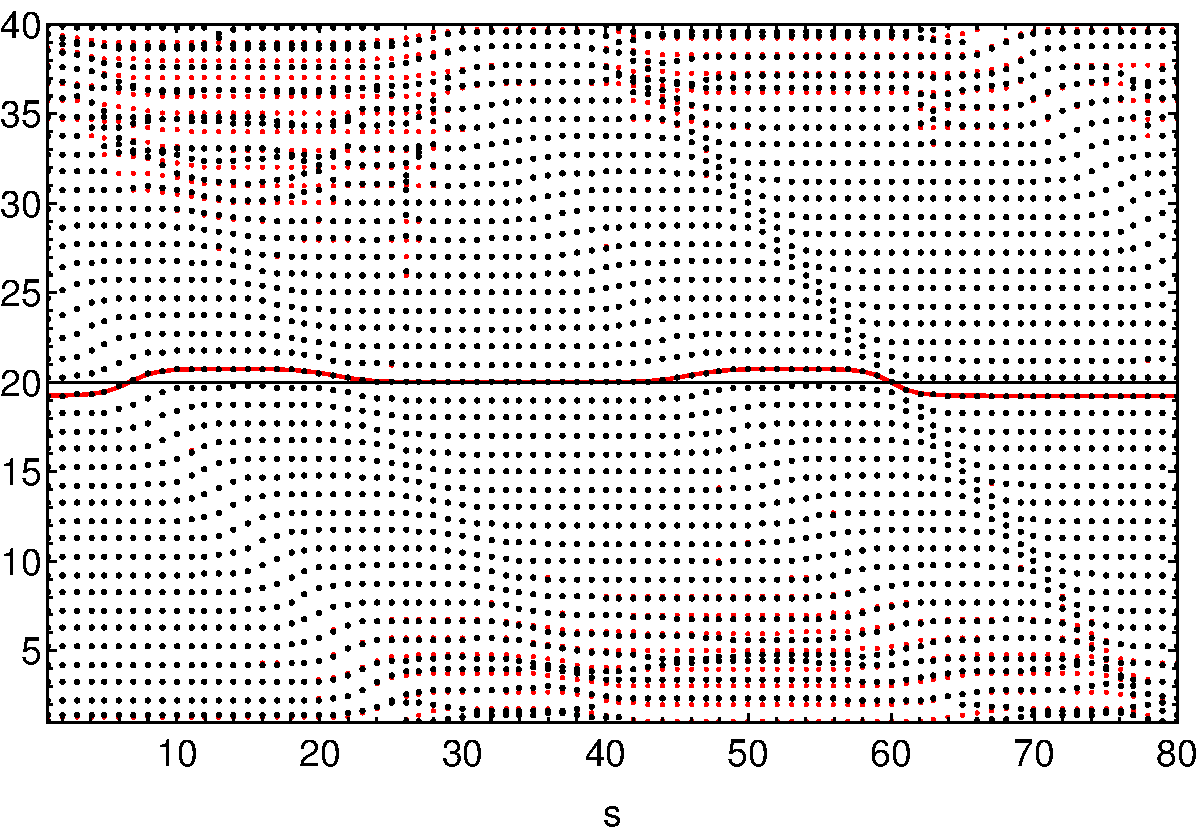
\includegraphics[width=90mm]{loca.pdf}
}}\hspace{0mm}

\makebox[0pt]{
\subfloat[$\chi_s$]{
  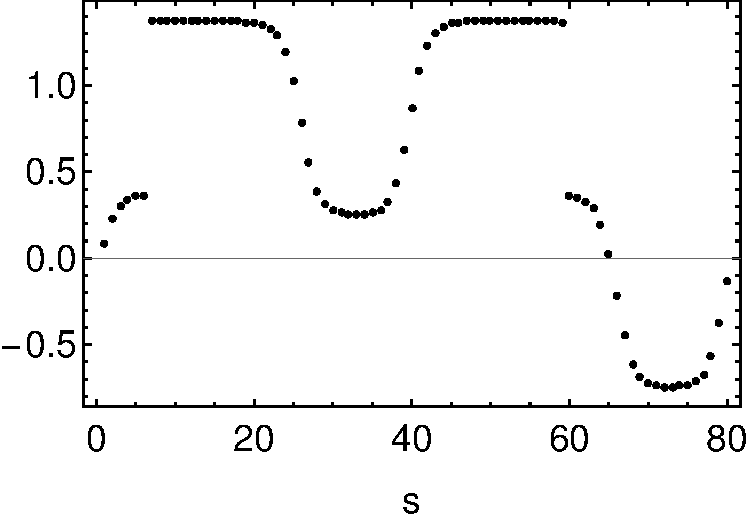
\includegraphics[width=45mm]{wan1.pdf}
}
\subfloat[$\chi_s'$ ]{
  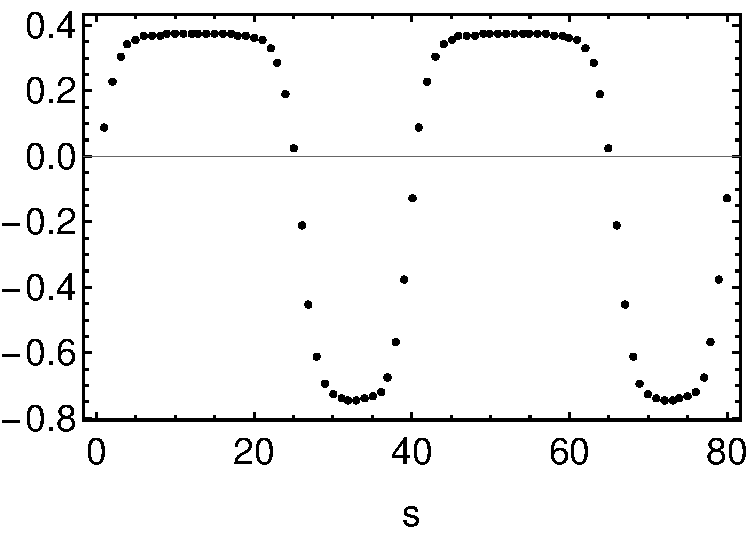
\includegraphics[width=45mm]{wan2.pdf}
}
}

\caption{a)Profile used for the inhomogeneous part $\kappa_s$. b,c,d) ES (black), $\chi_s$ mod $1$ (green), $\gamma$ (red), $\expval{\chi_s}_{\rm cuts}$ mod $1$ (dashed blue).}
\label{wan}
\end{figure}


\section{Superconducting systems}

The proof in Ref.\cite{Zaletel2014} also breaks down for superconducting systems. However, as we did for systems without translational invariance, one can extend expression \ref{mainl} for systems with pairing terms as well. Since one computes the Zak phase from the single-particle Bogoliubov-de Gennes Hamiltonian, we can obtain the correspondent entanglement spectrum and use expression \ref{mainl} to obtain the Zak phase. Take for example the kitaev chain, with the following Hamiltonian
\begin{align*}
H =& -\mu \sum_{i} c_i^\dagger c_i - t \sum_{i}\left( c_{i+1}^\dagger c_i + {\rm h.c.}\right) \\
&+  \sum_{i}\left( \Delta c_{i} c_{i+1} + {\rm h.c.}\right).
\end{align*}
Using the spinor $\phi_i^\dagger = (c_i^\dagger, c_i)$, we can rewrite the Hamiltonian as
\begin{align*}
&H = \frac{1}{2}\sum_i \phi^\dagger_i H_{BdG,ij} \phi_j,\\
&H_{BdG,ij} = -\mu \tau_z \delta_{ij} - (t \tau_z + i\Delta \tau_y )\delta_{i,j+1}- (t \tau_z - i\Delta \tau_y)\delta_{i,j-1}.
\end{align*}
Note that by taking $t' = \kappa = \kappa = 0$ in the BDI model, Eq. \ref{bdi_model}, we obtain
\begin{align*}
H_{ij} =& m \sigma_x\delta_{ij} + \frac{1}{2} t \left[(\sigma_x + i \sigma_y)\delta_{i,j+1} + (\sigma_x - i \sigma_y) \delta_{i,j-1} \right],
\end{align*}
which is just the Bogoliubov-de Gennes Hamiltonian of the Kitaev chain by rotating $x$ into $z$ and identifying $\mu = -m, t_{\rm Kit} = -t_{BDI}/2, \Delta = -t_{BDI}/2 $. From Fig.\ref{bdi_phase_diagram} we see that the $BDI$ model transitions from $\nu = 1$ to the trivial phase at $t=0, m=\pm t_{BDI}$, or alternatively, when $\mu = \pm 2 t_{Kit}$, which is the known result for the Kitaev chain. Therefore the results already shown for the BDI model studied here are also applicable to the Kitaev chain.  


\bibliography{references}	

	
\appendix

\section{Appendix A}
	
Consider a chain with periodic boundary conditions. A Schmidt decomposition for two bipartite cuts gives the ground state
\begin{equation}
\ket{\psi} = \sum_{p,q} \ket{p,q}_A s_p \ket{p,q}_B s_q,
\end{equation}
where we assume that the size of each subsystem is big enough so that the cuts can be considered independent of each other. We can now take subsystem B and glue its ends together to obtain the ground state of a ring with a single cut. If we include a flux threading inside the ring we obtain
\begin{equation}
\ket{\psi^\phi} = \sum_p s_p \ket{p,p}_B e^{i\phi Q_p},
\end{equation}
The many-body states $\ket{p,p}_B$ can be built by occupying the different ES eigenstates and are therefore characterized by a set of occupying numbers $\{n\}_p$. The many-body entanglement spectrum can also be expressed in terms of the single-particle one \cite{Alexandrinata2011} as
\begin{align}
s_p^2 =& \prod_{i \in {\rm occ}} \xi_i \prod_{i \in {\rm empty}}(1-\xi_i) \\
=& \prod_i (1-\xi_i)\left(\frac{\xi_i}{1-\xi_i} \right)^{n_i}
\end{align}
And the charge can be assigned so that $Q_p = \sum_{\alpha = b,l,r} q_\alpha\sum_{i \in \alpha} n_i$ with the constrain that $q_r,\pm q_b = q_l-1$ \textcolor{red}{Why?}. As the main result of \cite{Zaletel2014} the Zak phase is then found to be
\begin{align}
e^{i\gamma} = e^{2\pi i \sum_p s_p^2 Q_p}  \bra{\psi^0}\ket{\psi^{2\pi}},
\label{zaletel}
\end{align}
where the monodromy is given by
\begin{align}
\bra{\psi^0}\ket{\psi^{2\pi}} =& \sum_p s_p^2 e^{2\pi i Q_p}.
\end{align}
Consider the exponential term
\begin{align*}
e^{2\pi i (q_L N^p_l + (1-q_l)(N^p_r+N^p_b))} =& e^{2\pi i (q_l N^p_l + (1-q_l)(N-N^p_l))} \\
=& e^{4\pi i q_l N^p_l}e^{2 \pi i (N-N^p_l)}e^{-2\pi i q_l N },
\end{align*}
where $N^p_\alpha = \sum_{i \in \alpha} n_i$ and the total number of electrons, $N = \sum_{\alpha = b,l,r} N^p_\alpha$, is independent of $p$. We will consider two natural choices, $q_l = 1,1/2$, for which we have
\begin{align}
\bra{\psi^0}\ket{\psi^{2\pi}} =& 
\begin{cases}
1 & \text{for} \quad q_l = 1 \\
e^{N\pi i} & \text{for} \quad q_l = 1/2,
\end{cases}
\end{align}
where we used that $\sum_p s_p^2 = 1$. The change in the monodromy between both choices is accompanied by a change in the exponential term in Eq.\ref{zaletel}, so that both charge choices are equivalent.

Expressing the contribution of the many-body entanglement spectrum to the Zak phase in terms of the ES, we have
\begin{align*}
\gamma' = 2\pi \sum_{n_i = 0,1} \left(\sum_{i } n_i q_i\right) \left(\prod_m (1- \xi_m)\left(\frac{\xi_m}{1-\xi_m} \right)^{n_m} \right) ,
\end{align*} 
Consider now its derivative with respect to a particular entanglement eigenvalue
\begin{align}
\frac{1}{2\pi}\frac{\partial \gamma'}{\partial \xi_p} =& \sum_{\{n_k\}=0,1}\left(\sum_{i } n_i q_i\right)\frac{n_p - \xi_p}{\xi_p^{1-n_p}(1-\xi_p)^{n_p}}\\
&\times \left(\prod_{m\neq p} (1- \xi_m)\left(\frac{\xi_m}{1-\xi_m} \right)^{n_m} \right)
\end{align}
where
\begin{equation}
 \frac{n_p - \xi_p}{\xi_p^{1-n_p}(1-\xi_p)^{n_p}} = 
  \begin{cases}
    -1, & \text{for } n_p=0 \\
    1, & \text{for } n_p = 1 \\
  \end{cases}	
\end{equation}
Therefore we have
\begin{align*}
\frac{1}{2\pi}\frac{\partial \gamma'}{\partial \xi_p} =& -\sum_{\substack{\{n_{k\neq p}\}=0,1 \\ n_p = 0}}\left(\sum_{i \neq p} n_i q_i\right)\prod_{m\neq p} (1-\xi_m)\left( \frac{\xi_m}{1-\xi_m} \right)^{n_m} \\
&+ \sum_{\substack{\{n_{k\neq p}\}=0,1 \\ n_p = 1}}\left(\sum_{i \neq p} n_i q_i +q_p\right) \prod_{m\neq p} (1-\xi_m)\left( \frac{\xi_m}{1-\xi_m} \right)^{n_m} \\
=&q_p\sum_{\{n_{k\neq p}\}=0,1} \prod_{k\neq p} (1-\xi_k)\left( \frac{\xi_k}{1-\xi_k} \right)^{n_k} \\
\end{align*}
Expand now the sum  for another occupation number $n_{p'} = 0,1$ 
\begin{align*}
\frac{1}{2\pi}\frac{\partial \gamma'}{\partial \xi_p} =& q_p\sum_{\substack{n_{k \neq p \neq p'}=0,1\\ n_{p'}= 0}} (1-\xi_{p'})\prod_{k\neq p,p'} (1-\xi_k)\left( \frac{\xi_k}{1-\xi_k} \right)^{n_k} \\
&+ q_p\sum_{\substack{n_{k \neq p \neq p'}=0,1\\ n_{p'}= 1}} \xi_{p'}\prod_{k\neq p,p'} (1-\xi_k)\left( \frac{\xi_k}{1-\xi_k} \right)^{n_k} \\
 &=q_p\sum_{\substack{n_{k \neq p \neq p'}=0,1}} \prod_{k\neq p,p'} (1-\xi_k)\left( \frac{\xi_k}{1-\xi_k} \right)^{n_k} 
\end{align*}
doing this for the rest of the occupation numbers we obtain 
\begin{equation}
\frac{1}{2\pi}\frac{\partial \gamma'}{\partial \xi_p} = q_p,
\end{equation}
so that 
\begin{align*}
\gamma =& \gamma' - i\log(\bra{\psi^0}\ket{\psi^{2\pi}})\\
=& \sum_{i}q_i \xi_i - i\log(\bra{\psi^0}\ket{\psi^{2\pi}})\\
\end{align*}
and we have recovered equation \ref{mainl}. 

\end{document}